\section{Entraînement avec les hyperparamètres optimaux}%
\label{sec.results.retrain}

Après le réglage des hyperparamètres, nous avons entraîné le modèle en spécifiant un nombre maximal d'époques de 20.
L'entraînement s'est fait interrompu par le rappel de fonction \verb|EarlyStopping| après 9 époques.
Cela est dû au fait que le score \gls{bleu} sur le corpus de validation n'a pas augmenté pendant 3 époques consécutives.
L'exécution a duré 1h~26min~27s.

\begin{figure}[hbt]
    \begin{subfigure}{.5\textwidth}
        \caption{Exactitude}
        \begin{center}
            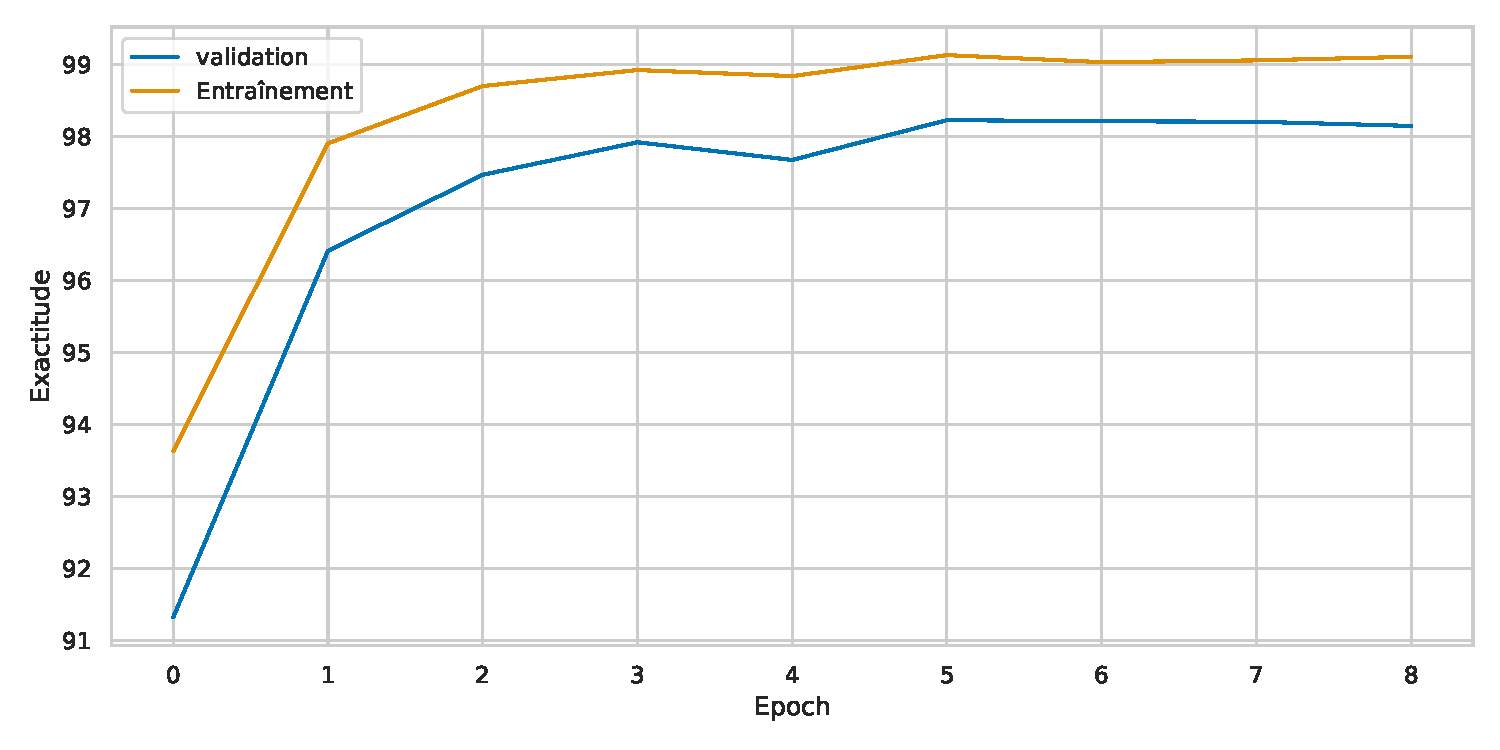
\includegraphics[width=\textwidth]{assets/python/tuned-accuracy.pdf}
        \end{center}
        \label{fig.results.tuned.training.accuracy}
    \end{subfigure}
    \begin{subfigure}{.5\textwidth}
        \caption{\glsfmtshort{bleu}}
        \begin{center}
            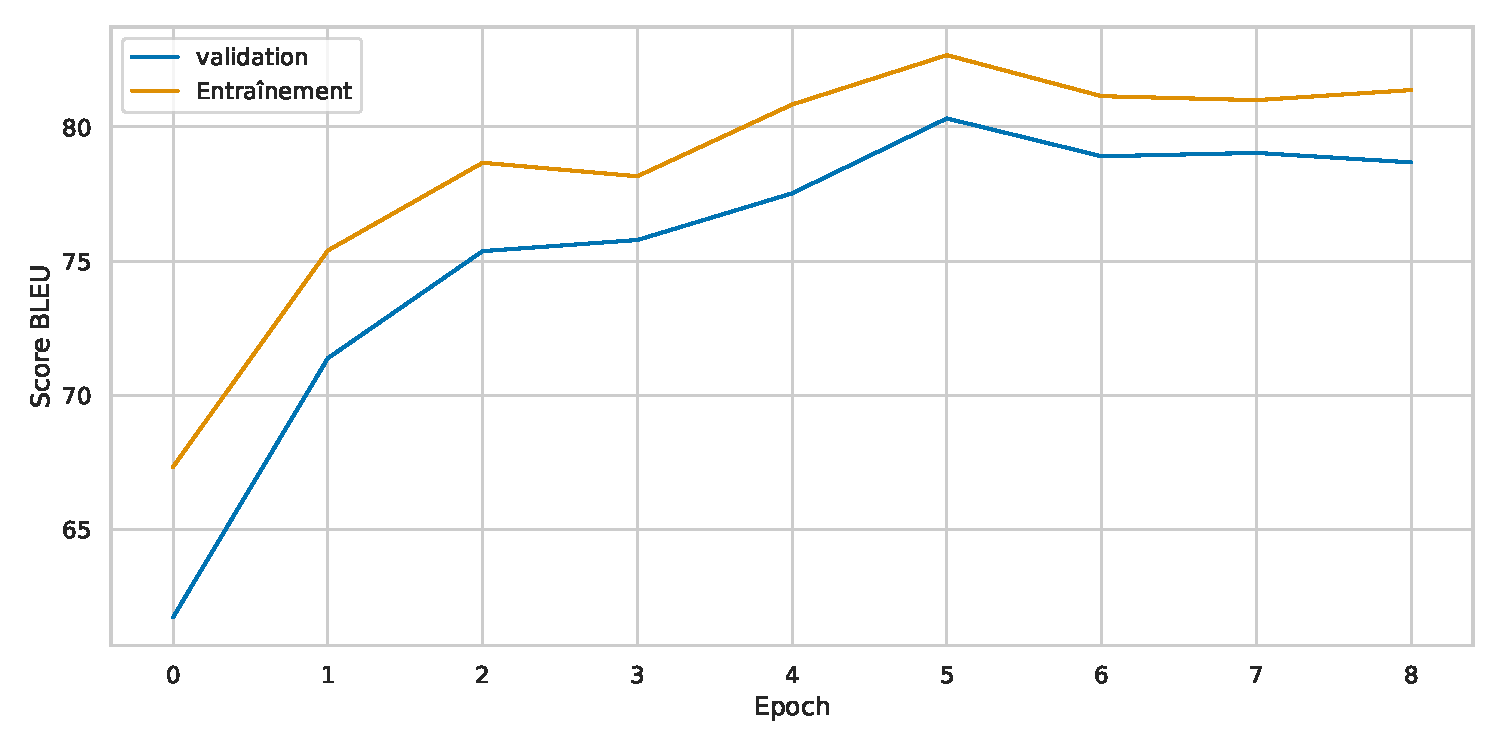
\includegraphics[width=\textwidth]{assets/python/tuned-bleu.pdf}
        \end{center}
        \label{fig.results.tuned.training.bleu}
    \end{subfigure}
    \begin{subfigure}{.5\textwidth}
        \begin{center}
            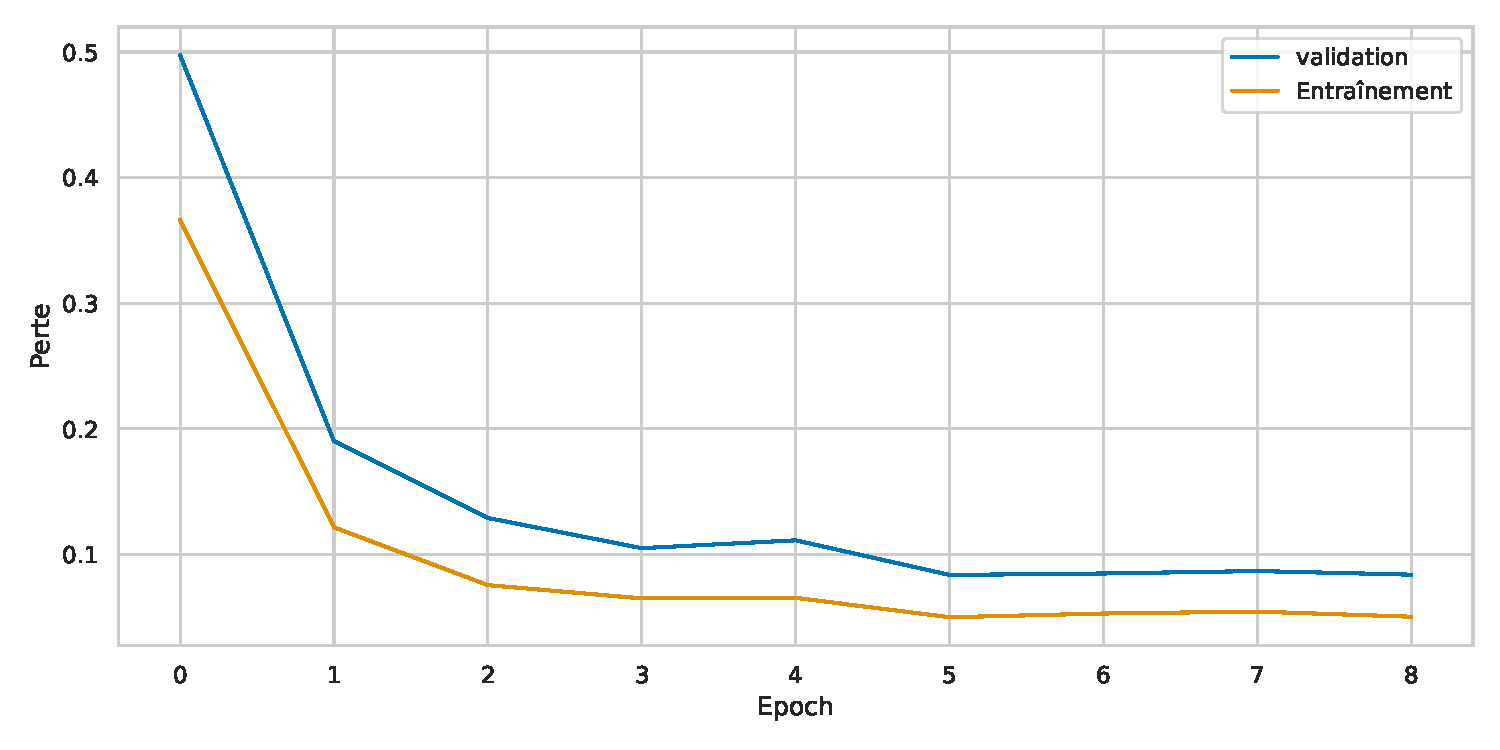
\includegraphics[width=\textwidth]{assets/python/tuned-loss.pdf}
        \end{center}
        \caption{Perte}
        \label{fig.results.tuned.training.loss}
    \end{subfigure}
    \caption{Évolution des métriques avec les hyperparamètres optimaux.}
    \label{fig.results.tuned.training}
\end{figure}
